\documentclass[11pt]{article}

\usepackage[a4paper,margin=2.35cm]{geometry}
\usepackage[T1]{fontenc}
\usepackage[utf8]{inputenc}
\usepackage{lmodern}
\usepackage{microtype}
\usepackage{amsmath,amssymb}
\usepackage{booktabs}
\usepackage{enumitem}
\usepackage{listings}
\usepackage{tikz}
\usepackage{hyperref}
\usepackage{xcolor}
\usetikzlibrary{arrows.meta,positioning,fit}

\hypersetup{
  pdftitle={Walrus Memory Graphs: Bitemporal Hypertext for Persistent AI Agents on Sui and Walrus},
  pdfauthor={[Author]},
  colorlinks=true,
  linkcolor=black,
  citecolor=black,
  urlcolor=black
}

\lstset{
  basicstyle=\ttfamily\small,
  breaklines=true,
  frame=single,
  columns=fullflexible,
  showstringspaces=false
}

\title{\textbf{Walrus Memory Graphs: Bitemporal Hypertext for Persistent AI Agents on Sui and Walrus}\\
\large Typed \texttt{wal://} Links Between Evolving Social Entities and Immutable Episodes}
\author{Daniel Devatman Hromada}
\date{September 2026}

\begin{document}
\maketitle

\begin{abstract}
Contemporary conversational agents usually treat memory as a collection of text fragments or vectors retrieved by semantic similarity. This is useful for recall, but it poorly represents identity, temporal evolution, provenance, and relationships among memories. We propose the \emph{Walrus Memory Graph}: a persistent, typed, hypertext-like memory architecture that combines mutable Sui objects with immutable Walrus blobs. Stable social entities---initially persons and Matrix rooms---receive persistent Sui object identifiers. Their changing descriptions are stored as append-only Walrus revisions, with the Sui object pointing to the current head. Episodic memories are immutable Walrus documents encoding what happened, when and where it happened, and who participated. Episodes refer to persons and rooms through an application-level URI scheme such as \texttt{wal://person/<sui-object-id>} and \texttt{wal://room/<sui-object-id>}. Each episode may additionally pin the exact interpersonal-memory revision that was current when the episode occurred. This produces a bitemporal graph in which an agent can ask both ``what do I know about this person now?'' and ``what did I know about this person when this event occurred?'' The design preserves historical lineage, supports cryptographic verification of stored states, and can keep sensitive social structure encrypted. We describe the data model, resolution semantics, update protocol, privacy model, concurrency rules, and a Matrix-native reference implementation suitable for persistent multi-user AI agents.
\end{abstract}

\section{Introduction}

Long-lived AI agents need more than retrieval. They need a notion of \emph{continuing identity}: the ability to recognize that a human encountered today is the same human encountered months earlier, that a conversational room has accumulated its own culture and history, and that an event belongs to a particular moment in the evolving relationship among these entities.

Most current agent-memory systems reduce this problem to a searchable store of textual memories or embedding vectors. Such systems can retrieve relevant fragments, but they make several important questions awkward:

\begin{itemize}[nosep]
    \item Which memories describe the same persistent person or social space?
    \item How did the agent's understanding of that person change over time?
    \item Which exact version of a person's memory informed an action in a past episode?
    \item Can old memories remain verifiable rather than being silently overwritten?
    \item Can an episode link directly to the people and rooms involved, as a hypertext document links to other documents?
\end{itemize}

This paper proposes a simple answer based on the complementary semantics of Sui and Walrus. Sui objects provide persistent identity: an object's contents may evolve while its object ID remains stable~\cite{sui}. Walrus provides immutable content-addressed storage: changed stored bytes produce a new blob identifier, leaving the previous version independently addressable~\cite{walrus-lineage,walrus-whitepaper}. The combination yields a natural division of labor:

\begin{quote}
\textbf{Sui represents what persists. Walrus represents what happened to be true at a particular revision.}
\end{quote}

We call the resulting structure a \emph{Walrus Memory Graph}. It borrows from the original hypertext idea of traversable associative structures~\cite{bush,nelson}, from episodic-memory theory~\cite{tulving}, and from recent agent architectures that treat memory as a first-class component~\cite{generative-agents,memgpt}. Unlike a conventional knowledge graph, however, the proposed graph explicitly combines mutable identity nodes with immutable historical states.

The motivating implementation is a Matrix-native conversational agent, here called \emph{Walden}. Matrix is useful because users, rooms and events already possess protocol-level identifiers~\cite{matrix-spec}. Nevertheless, the architecture is not Matrix-specific: Matrix supplies the social substrate, while Sui and Walrus supply the persistent memory substrate.

The contribution is therefore not merely ``put chatbot memories on decentralized storage.'' The contribution is a typed, temporal addressing model in which memory becomes navigable hypertext.

\section{Design Principles}

The architecture follows six principles.

\paragraph{Persistent identity.}
A person or social room should keep the same logical identity even when the agent's beliefs about it change. We therefore assign each such entity a stable Sui object.

\paragraph{Immutable historical state.}
A past description should never be overwritten. Every revision is stored as a new Walrus blob. Walrus blob IDs act as immutable handles to stored bytes~\cite{walrus-lineage}.

\paragraph{Typed references.}
Memories should refer to one another explicitly rather than only by semantic similarity. We define a small \texttt{wal://} namespace for persons, rooms, episodes and raw blobs.

\paragraph{Dual temporal access.}
The graph should support both current-state queries and historical-state queries. A stable person reference resolves to the current head, while a pinned blob reference resolves to the exact historical revision.

\paragraph{Privacy by encryption.}
Walrus blobs are publicly retrievable when their blob IDs are known unless the application encrypts them. Sensitive memories must therefore be encrypted before storage; Walrus Memory supports Seal-based encryption~\cite{walrus-agent-loop,walrus-console}.

\paragraph{Sparse use of on-chain state.}
Not every memory requires a Sui object. Stable entities receive Sui identities; high-volume episodic records remain inexpensive immutable Walrus blobs. This keeps the chain as an identity and head-pointer layer rather than a transcript database.

\section{Memory Types}

We initially distinguish three memory types.

\subsection{Interpersonal memory: who}

An \emph{interpersonal memory} represents the agent's evolving model of a human counterpart. It may contain stable facts, preferences, shared history, projects, unresolved topics, confidence values and provenance links. It is not the human being itself; it is explicitly the agent's current memory \emph{of} that human.

For each known person $p$, the system creates a Sui object $O_p$ with stable identifier $id(O_p)$. The object's principal mutable field is a head pointer

\[
H(O_p) = b_k,
\]

where $b_k$ is the Walrus blob ID of the latest interpersonal-memory revision.

Each revision contains a link to its predecessor:

\[
P(b_k)=b_{k-1}, \qquad P(b_0)=\bot.
\]

Thus the current Sui object identifies the latest state, while repeated application of $P$ reconstructs the complete retained lineage.

\subsection{Room memory: social context}

A Matrix room is more than a bag of messages. Long-running rooms accumulate topics, norms, roles, recurring projects, inside references, shared decisions and characteristic interaction patterns. We therefore introduce a second persistent entity type: \emph{room memory}.

A Matrix room known to the agent receives a stable Sui object $O_r$. Its current Walrus head contains the agent's evolving model of that room. The public Sui object need not contain the literal Matrix room ID. The binding between a Matrix room ID and its Sui memory object can remain local or encrypted.

Room memory may include references to interpersonal memories, for example the recurrent participants of the room:

\begin{lstlisting}
{
  "schema": "walden-room-memory/1",
  "previous": "wal://blob/<previous-room-memory-blob>",
  "topic": "...",
  "shared_context": ["..."],
  "norms": ["..."],
  "participants": [
    "wal://person/0x...",
    "wal://person/0x..."
  ],
  "open_threads": ["..."]
}
\end{lstlisting}

\subsection{Episodic memory: what, where and when}

An \emph{episodic memory} represents an event situated in time and context. In the spirit of Tulving's distinction between episodic and semantic memory~\cite{tulving}, an episode is not primarily a timeless fact. It records that something happened.

A minimal episode answers:

\begin{center}
\textbf{what happened? \quad when? \quad where/in which room? \quad who was involved?}
\end{center}

Episodes are high-volume and naturally append-only, so the default representation is a Walrus blob rather than a Sui object. An episode can directly reference the stable persons and rooms involved.

\begin{lstlisting}
{
  "schema": "walden-episode/1",
  "when": {
    "start": "2026-09-22T11:14:00+02:00",
    "end":   "2026-09-22T12:03:00+02:00"
  },
  "room": "wal://room/0x...",
  "where": {
    "kind": "virtual",
    "label": "Matrix conversation"
  },
  "what": {
    "type": "conversation",
    "summary": "Discussion of persistent agent memory graphs"
  },
  "who": [
    {
      "person": "wal://person/0x...",
      "memory_at_time": "wal://blob/<person-revision-A>"
    },
    {
      "person": "wal://person/0x...",
      "memory_at_time": "wal://blob/<person-revision-B>"
    }
  ],
  "related": []
}
\end{lstlisting}

The paired fields \texttt{person} and \texttt{memory\_at\_time} are central to the design. The first identifies the person diachronically. The second freezes the agent's knowledge of that person at the moment of the episode.

\section{The \texttt{wal://} Hypertext Namespace}

We define an application-level URI convention:

\begin{lstlisting}
wal://person/<sui-object-id>
wal://room/<sui-object-id>
wal://episode/<walrus-blob-id>
wal://blob/<walrus-blob-id>
\end{lstlisting}

This is a Walden/Walrus-Memory-Graph convention, not an official Walrus URI scheme. Its purpose is to give stored memories typed, traversable references. The type component determines how the identifier is resolved.

\begin{table}[h]
\centering
\caption{Resolution semantics of the proposed \texttt{wal://} namespace.}
\begin{tabular}{lll}
\toprule
Type & Identifier & Resolution \\
\midrule
\texttt{person} & Sui object ID & read Sui object $\rightarrow$ current Walrus head \\
\texttt{room} & Sui object ID & read Sui object $\rightarrow$ current Walrus head \\
\texttt{episode} & Walrus blob ID & retrieve immutable episode blob \\
\texttt{blob} & Walrus blob ID & retrieve exact immutable blob \\
\bottomrule
\end{tabular}
\end{table}

The namespace deliberately mixes two kinds of identifiers, but never ambiguously: the URI type tells the resolver whether the following identifier belongs to Sui or Walrus.

For a stable entity $x$, current-state resolution is

\[
R_t(\texttt{wal://person/}x)=\operatorname{WalrusGet}(H_t(x)).
\]

By contrast,

\[
R(\texttt{wal://blob/}b)=\operatorname{WalrusGet}(b)
\]

is temporally invariant for as long as the blob remains retained and retrievable.

\section{A Bitemporal Memory Graph}

The combination of stable references and pinned historical references creates a useful form of bitemporality.

Consider an episode $e$ involving Alice. The episode stores both

\begin{lstlisting}
"person": "wal://person/<alice-sui-id>"
\end{lstlisting}

and

\begin{lstlisting}
"memory_at_time": "wal://blob/<alice-v4>"
\end{lstlisting}

Months later, Alice's Sui person object may point to revision $v_{17}$. The same old episode can now answer two distinct queries:

\begin{description}[style=nextline]
\item[What does the agent know about Alice now?]
Resolve \texttt{wal://person/<alice-sui-id>} through the current Sui head.

\item[What did the agent know about Alice during this episode?]
Resolve the pinned \texttt{wal://blob/<alice-v4>} reference.
\end{description}

This distinction matters because agent memory is epistemic, not merely archival. A later correction should change present belief without rewriting what the agent actually believed in the past.

Formally, let $E$ be the set of stable entities, $B$ the set of immutable Walrus revisions, and $Q$ the set of episodes. At time $t$ the memory graph is

\[
G_t=(V,\mathcal{E}_t), \qquad V=E\cup B\cup Q.
\]

Important edge types include:

\begin{align*}
\textsf{head}_t &: E \rightarrow B,\\
\textsf{previous} &: B \rightarrow B\cup\{\bot\},\\
\textsf{participant} &: Q \rightarrow E,\\
\textsf{snapshot} &: Q \rightarrow B,\\
\textsf{room} &: Q \rightarrow E,\\
\textsf{related} &: Q \rightarrow Q\cup B.
\end{align*}

Only \textsf{head} is intrinsically mutable. The remaining historical edges are append-only once written.

\section{Architecture}

Figure~\ref{fig:graph} shows a minimal graph with two people, one Matrix room and one episode.

\begin{figure}[h]
\centering
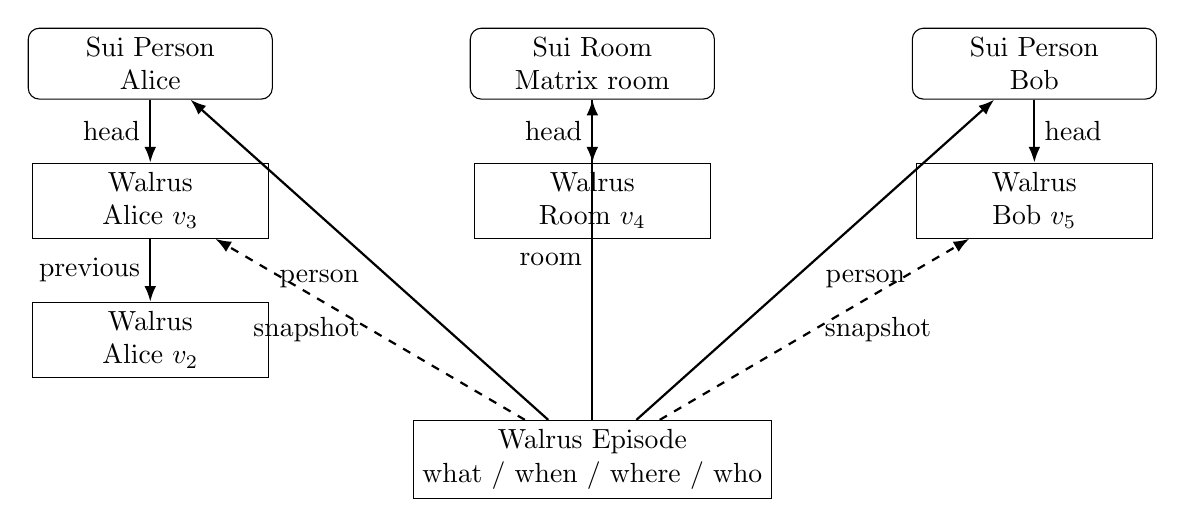
\begin{tikzpicture}[
    node distance=8mm and 14mm,
    sui/.style={draw,rounded corners,align=center,minimum width=31mm,minimum height=9mm},
    wal/.style={draw,align=center,minimum width=30mm,minimum height=9mm},
    arr/.style={-{Latex[length=2mm]},thick}
]
\node[sui] (alice) {Sui Person\\Alice};
\node[wal,below=of alice] (a3) {Walrus\\Alice $v_3$};
\node[wal,below=of a3] (a2) {Walrus\\Alice $v_2$};

\node[sui,right=25mm of alice] (room) {Sui Room\\Matrix room};
\node[wal,below=of room] (r4) {Walrus\\Room $v_4$};

\node[sui,right=25mm of room] (bob) {Sui Person\\Bob};
\node[wal,below=of bob] (b5) {Walrus\\Bob $v_5$};

\node[wal,below=23mm of r4] (ep) {Walrus Episode\\what / when / where / who};

\draw[arr] (alice) -- node[left]{head} (a3);
\draw[arr] (a3) -- node[left]{previous} (a2);
\draw[arr] (room) -- node[left]{head} (r4);
\draw[arr] (bob) -- node[right]{head} (b5);
\draw[arr] (ep) -- node[below left]{person} (alice);
\draw[arr] (ep) -- node[left]{room} (room);
\draw[arr] (ep) -- node[below right]{person} (bob);
\draw[arr,dashed] (ep) -- node[left]{snapshot} (a3);
\draw[arr,dashed] (ep) -- node[right]{snapshot} (b5);
\end{tikzpicture}
\caption{A Walrus Memory Graph combines stable Sui entity identities with immutable Walrus state and episode nodes. Solid entity-head edges resolve current state; pinned snapshot edges preserve historical epistemic state.}
\label{fig:graph}
\end{figure}

This architecture has an intentionally asymmetric topology. Persons and rooms are \emph{entities}; episodes are \emph{occurrences}. Entities need stable identity and mutable heads. Occurrences normally need only immutable storage.

\section{Update Protocol}

\subsection{First encounter}

When the agent encounters a previously unknown Matrix user, it performs the following conceptual procedure:

\begin{enumerate}[nosep]
    \item Create an initial encrypted interpersonal-memory document $m_0$ with \texttt{previous = null}.
    \item Store $m_0$ on Walrus and obtain blob ID $b_0$.
    \item Create a Sui person-memory object whose head equals $b_0$.
    \item Store the Matrix-user-ID $\leftrightarrow$ Sui-object-ID binding in a private local or encrypted identity index.
\end{enumerate}

The public Sui object therefore need not reveal the Matrix identifier.

\subsection{Interpersonal-memory revision}

Suppose the current head of person object $O_p$ is $b_k$. To incorporate new information:

\begin{enumerate}[nosep]
    \item Retrieve and decrypt $b_k$.
    \item Derive the new memory state $m_{k+1}$.
    \item Set \texttt{previous = wal://blob/$b_k$}.
    \item Encrypt and store $m_{k+1}$ on Walrus, yielding $b_{k+1}$.
    \item Atomically change $H(O_p)$ from $b_k$ to $b_{k+1}$.
\end{enumerate}

The old revision remains addressable and can be reached by following \texttt{previous} links.

\subsection{Optimistic concurrency}

A social agent may operate in several Matrix rooms simultaneously. Two workers could therefore read the same head and attempt concurrent updates. The Move update function should include an expected-parent guard:

\begin{lstlisting}
update_head(person_object,
            expected_head = old_blob_id,
            new_head      = new_blob_id)
\end{lstlisting}

The transaction succeeds only if the current head still equals \texttt{expected\_head}. Otherwise the worker reloads the newer state and rebases or merges its proposed update. This prevents a last-writer-wins race from silently deleting memory.

\subsection{Episode creation}

For each meaningful episode, the agent resolves every participant's current person head and the room's current head. The episode stores stable references and, where useful, pinned revision references. The episode is then encrypted and written as a new Walrus blob.

Crucially, an episode does not have to cause a new interpersonal revision. Observation and consolidation are separate operations. A high-volume conversation can therefore produce many episodes while interpersonal state is updated only when a durable fact, preference or relationship-level interpretation changes.

\section{Memory as Hypertext}

The architecture revives a central idea from early hypertext: information is useful not only because it can be searched, but because it can be \emph{traversed} through meaningful links~\cite{bush,nelson}. Vector retrieval and graph traversal solve different problems.

A semantic query such as ``what did Alice say about sustainable AI?'' may begin with vector recall. Once an episode is found, however, typed links provide deterministic navigation:

\[
\text{episode}
\rightarrow \text{person}
\rightarrow \text{current interpersonal head}
\rightarrow \text{previous revisions}.
\]

Or:

\[
\text{episode}
\rightarrow \text{room}
\rightarrow \text{current room memory}
\rightarrow \text{participants}.
\]

The graph therefore complements embeddings rather than replacing them. Embeddings answer \emph{which memory may be relevant?}; typed links answer \emph{what exactly is this memory connected to?}

This distinction is especially important for agentic behavior. An agent can use semantic recall to discover a relevant episode, then traverse explicit links to gather the people, room context and historically appropriate memory snapshots needed to interpret it.

\section{Epistemic Provenance}

A memory system should distinguish observations from inferences. Interpersonal memory can represent claims as structured assertions rather than unqualified prose:

\begin{lstlisting}
{
  "claim": "prefers concise technical explanations",
  "confidence": 0.86,
  "status": "active",
  "first_seen": "wal://episode/<...>",
  "last_confirmed": "wal://episode/<...>",
  "sources": [
    "wal://episode/<...>",
    "wal://episode/<...>"
  ]
}
\end{lstlisting}

This turns the memory graph into an epistemic graph: durable beliefs can point back to the episodes from which they were inferred. Later corrections need not erase the old claim. A new revision can mark it as superseded while retaining the original provenance.

The same mechanism applies to room memory. A claim such as ``this room is mainly used for project X'' can be supported by a set of episode references and revised as the room evolves.

\section{Privacy and Access Control}

The architecture concerns human relationships and therefore treats privacy as a primary design constraint rather than an optional deployment detail.

\subsection{Encrypt all sensitive Walrus payloads}

Walrus storage should be assumed publicly readable when a blob ID is known. Walrus Memory supports Seal encryption, and client-managed encryption is available when plaintext must not be exposed to a relayer~\cite{walrus-agent-loop,walrus-console}. Person, room and episode documents should therefore be encrypted before they reach Walrus.

\subsection{Do not publish Matrix identities in Sui objects}

The stable Sui object should not contain a literal Matrix user ID or room ID. Nor is a plain unsalted hash necessarily sufficient: Matrix identifiers can be guessable. A private identity-binding layer should map Matrix identities to Sui memory objects.

Conceptually:

\begin{lstlisting}
private_identity_index:
  @alice:example.org  -> wal://person/0x...
  !room-id            -> wal://room/0x...
\end{lstlisting}

This mapping may live in an encrypted local database or in an encrypted Walrus document under a stricter access policy.

\subsection{Keep the social graph encrypted}

If episode participant lists and room participant lists are inside encrypted Walrus payloads, an outside observer can see that blobs and Sui objects exist without trivially reconstructing who interacted with whom. The graph is therefore logical rather than necessarily publicly legible.

\subsection{Deletion and forgetting}

Immutability must not be confused with eternal retention. Walrus storage is time-bounded and can be renewed; deletable blobs can also relinquish their Walrus storage allocation~\cite{walrus-whitepaper,walrus-console}. However, deletion from Walrus cannot guarantee erasure of copies already cached or replicated elsewhere. For sensitive human memory, application-level forgetting should therefore combine cryptographic key destruction, retention-policy expiration and minimization of what is written in the first place.

\section{Retention and Lineage}

A lineage is useful only while its referenced blobs remain retrievable. Walrus storage is purchased for bounded epochs and can be extended without re-uploading the blob~\cite{walrus-whitepaper}. A long-lived agent therefore requires a renewal policy.

Not every episode deserves indefinite retention. We propose three retention classes:

\begin{description}[style=nextline]
\item[Working episodes]
Short-lived, high-volume observations retained for a limited horizon.

\item[Consolidated episodes]
Events that support durable interpersonal or room knowledge; retained longer because they serve as provenance.

\item[Identity lineage]
Interpersonal and room revisions that remain reachable from current heads or historically important episodes; automatically renewed while needed.
\end{description}

This creates a memory ecology rather than an ever-growing transcript archive.

\section{Reference Implementation in Matrix}

The reference implementation uses Matrix as the interaction substrate. Matrix provides unique user and room identifiers, while rooms constitute durable conversational contexts~\cite{matrix-spec}. The agent maintains private bindings from Matrix IDs to the corresponding Sui memory objects.

A message-processing cycle can be organized as follows:

\begin{enumerate}
    \item Receive a Matrix event and resolve the sender to a \texttt{wal://person/...} identity.
    \item Resolve the Matrix room to a \texttt{wal://room/...} identity.
    \item Retrieve current interpersonal and room heads.
    \item Perform semantic recall from Walrus Memory for potentially relevant older episodes.
    \item Traverse typed references from recalled episodes to obtain exact entity context.
    \item Generate the agent response.
    \item Persist a new episodic memory if the interaction is meaningful.
    \item Consolidate durable changes into interpersonal and/or room lineages.
\end{enumerate}

Walrus Memory already provides a memory-oriented API with encryption, vector indexing and recall, and its documentation explicitly treats agent state as versionable Walrus data~\cite{walrus-lineage,walrus-memory-api}. The proposed graph layer adds typed identity, lineage heads and cross-memory references above these primitives.

For many small memories, Walrus Quilt-style batching can reduce transaction and storage overhead, although quilt patch identifiers have different lifecycle semantics and therefore should be introduced only after the basic graph model is validated~\cite{walrus-agent-loop}.

\section{Prototype Evaluation}

The first implementation is intended as a live Matrix chatbot and as a submission to the 2026 Walrus Sessions ``Chatbots That Remember'' hackathon. The evaluation should demonstrate memory doing visible work rather than existing as decorative storage.

We propose four tests.

\subsection{Cross-session interpersonal continuity}
A user tells the agent a durable preference in session $A$. In a later session $B$, the agent should resolve the same person object, retrieve its current interpersonal head, and apply the preference without requiring the user to repeat it.

\subsection{Room-specific continuity}
The same person interacts with the agent in two Matrix rooms with different norms or projects. The agent should retrieve the same person identity but different \texttt{wal://room/...} contexts.

\subsection{Historical epistemic reconstruction}
A fact about a person changes between two dates. A current query should return the latest interpersonal state; a query about an older episode should recover the pinned historical snapshot and therefore reconstruct what the agent knew at that time.

\subsection{Graph traversal after semantic recall}
A semantic query retrieves one episode through vector similarity. The agent then follows deterministic links from the episode to its participants and room rather than performing additional fuzzy searches for those identities.

Measurements should include end-to-end recall latency, number of Walrus writes, amount of on-chain Sui state, WAL storage cost, number of successful lineage traversals, and correctness of current-versus-historical queries. No performance values are reported here because the prototype evaluation is still to be executed.

\section{Discussion}

\subsection{Why not store everything in a vector database?}

A vector database is excellent at approximate relevance. It does not by itself provide persistent identity, exact historical references or typed relationships. The proposed system keeps vector recall, but treats it as an entrance into a more explicit memory structure.

\subsection{Why not store everything on Sui?}

Conversation-derived memory is high-volume and often text-heavy. Putting every episode on-chain would use Sui as a document database and would unnecessarily increase cost and public metadata. Sui is used only where its persistent-object semantics are valuable: stable entity identity, head pointers and access-policy coordination.

\subsection{Why not keep only the latest memory?}

Overwriting loses epistemic history. If an agent changes its belief about a person, a historical episode should still be interpretable according to the state available at that time. Immutable Walrus revisions preserve this distinction naturally.

\subsection{Why rooms as first-class entities?}

Human identity alone does not determine conversational meaning. The same participants behave differently in a research room, family room, project room or public community. A room therefore functions as a durable social context with its own evolving memory. Treating \texttt{wal://room/...} as a first-class entity lets the agent model this context without collapsing it into individual profiles.

\subsection{Beyond persons and rooms}

The namespace is extensible. Future entity types could include projects, places, organizations, artefacts or long-lived tasks. The important design rule is that a type receives a Sui identity only when stable identity and mutable state are genuinely required. Otherwise a Walrus blob is sufficient.

\section{Limitations and Open Questions}

Several issues require empirical study.

First, memory consolidation remains an AI problem: the storage layer can preserve revisions, but it does not decide which observations deserve to modify interpersonal or room memory. Second, conflict resolution becomes non-trivial when multiple agent processes update the same entity concurrently. Third, long-term retention has economic cost and requires renewal policy. Fourth, privacy depends on key management; encrypted memories become unrecoverable if keys are lost, while compromised keys expose potentially sensitive social data. Fifth, a stable Sui object can itself reveal metadata such as update frequency even when payloads are encrypted. Finally, the proposed \texttt{wal://} scheme is currently application-level and would need specification, canonical encoding rules and security review before interoperability across implementations.

These limitations are not reasons to collapse the architecture back into a flat vector store. They identify the engineering boundary between \emph{remembering something} and maintaining a durable, inspectable memory structure over time.

\section{Conclusion}

We proposed the Walrus Memory Graph, a hypertext-like architecture for persistent AI memory built from two complementary primitives. Sui objects provide stable mutable identities. Walrus blobs provide immutable, independently addressable states. Typed \texttt{wal://} references connect them.

The initial ontology is deliberately small. \emph{Interpersonal memories} answer \textbf{who}. \emph{Room memories} represent persistent social context. \emph{Episodic memories} answer \textbf{what, when, where, and with whom}. Episodes link to stable person and room identities and may simultaneously pin the exact historical memory revisions that were current when the episode occurred.

The result is more than persistent chatbot context. It is a temporal social hypertext in which an AI agent can traverse its own memory, distinguish present knowledge from past belief, and preserve the provenance of how its understanding developed. Walrus supplies the immutable pages; Sui supplies the persistent names; the graph emerges from the links between them.

\begin{thebibliography}{99}

\bibitem{bush}
V. Bush.
\newblock As We May Think.
\newblock \emph{The Atlantic Monthly}, 176(1):101--108, 1945.

\bibitem{nelson}
T. H. Nelson.
\newblock Complex Information Processing: A File Structure for the Complex, the Changing and the Indeterminate.
\newblock In \emph{Proceedings of the 20th ACM National Conference}, 1965.

\bibitem{tulving}
E. Tulving.
\newblock Episodic and Semantic Memory.
\newblock In E. Tulving and W. Donaldson, editors, \emph{Organization of Memory}. Academic Press, 1972.

\bibitem{generative-agents}
J. S. Park, J. O'Brien, C. J. Cai, M. R. Morris, P. Liang, and M. S. Bernstein.
\newblock Generative Agents: Interactive Simulacra of Human Behavior.
\newblock In \emph{Proceedings of the 36th Annual ACM Symposium on User Interface Software and Technology}, 2023.

\bibitem{memgpt}
C. Packer, S. Wooders, K. Lin, V. Fang, S. G. Patil, I. Stoica, and J. E. Gonzalez.
\newblock MemGPT: Towards LLMs as Operating Systems.
\newblock arXiv:2310.08560, 2023.

\bibitem{sui}
The MystenLabs Team.
\newblock The Sui Smart Contracts Platform.
\newblock Technical paper, Mysten Labs, 2022--2026 documentation edition.

\bibitem{walrus-whitepaper}
The MystenLabs Team.
\newblock Walrus: An Efficient Decentralized Storage Network.
\newblock Version 2.0, April 2025.

\bibitem{walrus-lineage}
Walrus Foundation.
\newblock Versioned Datasets and Lineage.
\newblock Walrus Memory Documentation, accessed September 2026.

\bibitem{walrus-agent-loop}
Walrus Foundation.
\newblock Agent Storage Loop.
\newblock Walrus Memory Documentation, accessed September 2026.

\bibitem{walrus-memory-api}
Walrus Foundation.
\newblock Walrus Memory SDK and Relayer API Reference.
\newblock Walrus Memory Documentation, accessed September 2026.

\bibitem{walrus-console}
Walrus Foundation.
\newblock Walrus Console: Encryption, Storage Epochs and Renewal.
\newblock Walrus Documentation, accessed September 2026.

\bibitem{matrix-spec}
The Matrix.org Foundation.
\newblock Matrix Specification: Identifier Grammar, Users, Rooms and URIs.
\newblock Matrix Specification, accessed September 2026.

\end{thebibliography}

\end{document}
